\documentclass[9pt,twocolumn,twoside,lineno]{pnas-new}
% Use the lineno option to display guide line numbers if required.

\templatetype{pnasresearcharticle} % Choose template 
% {pnasresearcharticle} = Template for a two-column research article
% {pnasmathematics} %= Template for a one-column mathematics article
% {pnasinvited} %= Template for a PNAS invited submission

\title{SARS-CoV-2 Genome surveillance in Switzerland: Can we quantify the effects of policy?}

% Use letters for affiliations, numbers to show equal authorship (if applicable) and to indicate the corresponding author
\author[a,c,1]{Author One}
\author[b,1,2]{Author Two} 
\author[a]{Author Three}

\affil[a]{Affiliation One}
\affil[b]{Affiliation Two}
\affil[c]{Affiliation Three}

% Please give the surname of the lead author for the running footer
\leadauthor{Lead author last name} 

% Please add a significance statement to explain the relevance of your work
\significancestatement{Authors must submit a 120-word maximum statement about the significance of their research paper written at a level understandable to an undergraduate educated scientist outside their field of speciality. The primary goal of the significance statement is to explain the relevance of the work in broad context to a broad readership. The significance statement appears in the paper itself and is required for all research papers.}

% Please include corresponding author, author contribution and author declaration information
\authorcontributions{Please provide details of author contributions here.}
\authordeclaration{Please declare any competing interests here.}
\equalauthors{\textsuperscript{1}A.O.(Author One) contributed equally to this work with A.T. (Author Two) (remove if not applicable).}
\correspondingauthor{\textsuperscript{2}To whom correspondence should be addressed. E-mail: author.two\@email.com}

% At least three keywords are required at submission. Please provide three to five keywords, separated by the pipe symbol.
\keywords{Keyword 1 $|$ Keyword 2 $|$ Keyword 3 $|$ ...} 

\begin{abstract}
% Please provide an abstract of no more than 250 words in a single paragraph. Abstracts should explain to the general reader the major contributions of the article. References in the abstract must be cited in full within the abstract itself and cited in the text.
Are the effects of policies designed to prevent and contain SARS-CoV-2 imports evident in genomic surveillance data? Here we use SARS-CoV-2 genome sequences from approximately 1\% of all confirmed cases in Switzerland from the first case on February 25th through December 31st 2020 to identify local transmission chains, estimate their international sources, and quantify their spread in Switzerland. We first performed a large-scale phylogenetic analysis to characterize the spatial and temporal pattern of virus imports into Switzerland and test for evidence whether Switzerland’s travel quarantine policy reduced virus imports. We then performed a phylodynamic analysis to quantify transmission chain spread in Switzerland and test whether Switzerland’s contact tracing program was able to slow the spread of imported lineages once local cases were identified. These analyses aim to help us understand the importance of international travel towards a national epidemic, an increasingly relevant topic as global vaccination campaigns continue at an uneven pace and new variants of concern spread internationally. 
\end{abstract}

\dates{This manuscript was compiled on \today}
\doi{\url{www.pnas.org/cgi/doi/10.1073/pnas.XXXXXXXXXX}}

\begin{document}

\maketitle
\thispagestyle{firststyle}
\ifthenelse{\boolean{shortarticle}}{\ifthenelse{\boolean{singlecolumn}}{\abscontentformatted}{\abscontent}}{}

% If your first paragraph (i.e. with the \dropcap) contains a list environment (quote, quotation, theorem, definition, enumerate, itemize...), the line after the list may have some extra indentation. If this is the case, add \parshape=0 to the end of the list environment.
% \dropcap{T}his PNAS journal template is provided to help you write your work in the correct journal format. Instructions for use are provided below. 
\dropcap{G}enomic data are useful for identifying transmission chains and their sources in the absence of linked epidemiological data.

\section*{Transmission chains composing the Swiss epidemic}

\subsection{Transmission chain longevity}
During the first wave, transmission chains are driven to extinction within a few months. During the second wave, similarly stringent policies do not succeed in driving transmission chains to extinction so quickly.

\begin{figure}[tbhp]
\centering
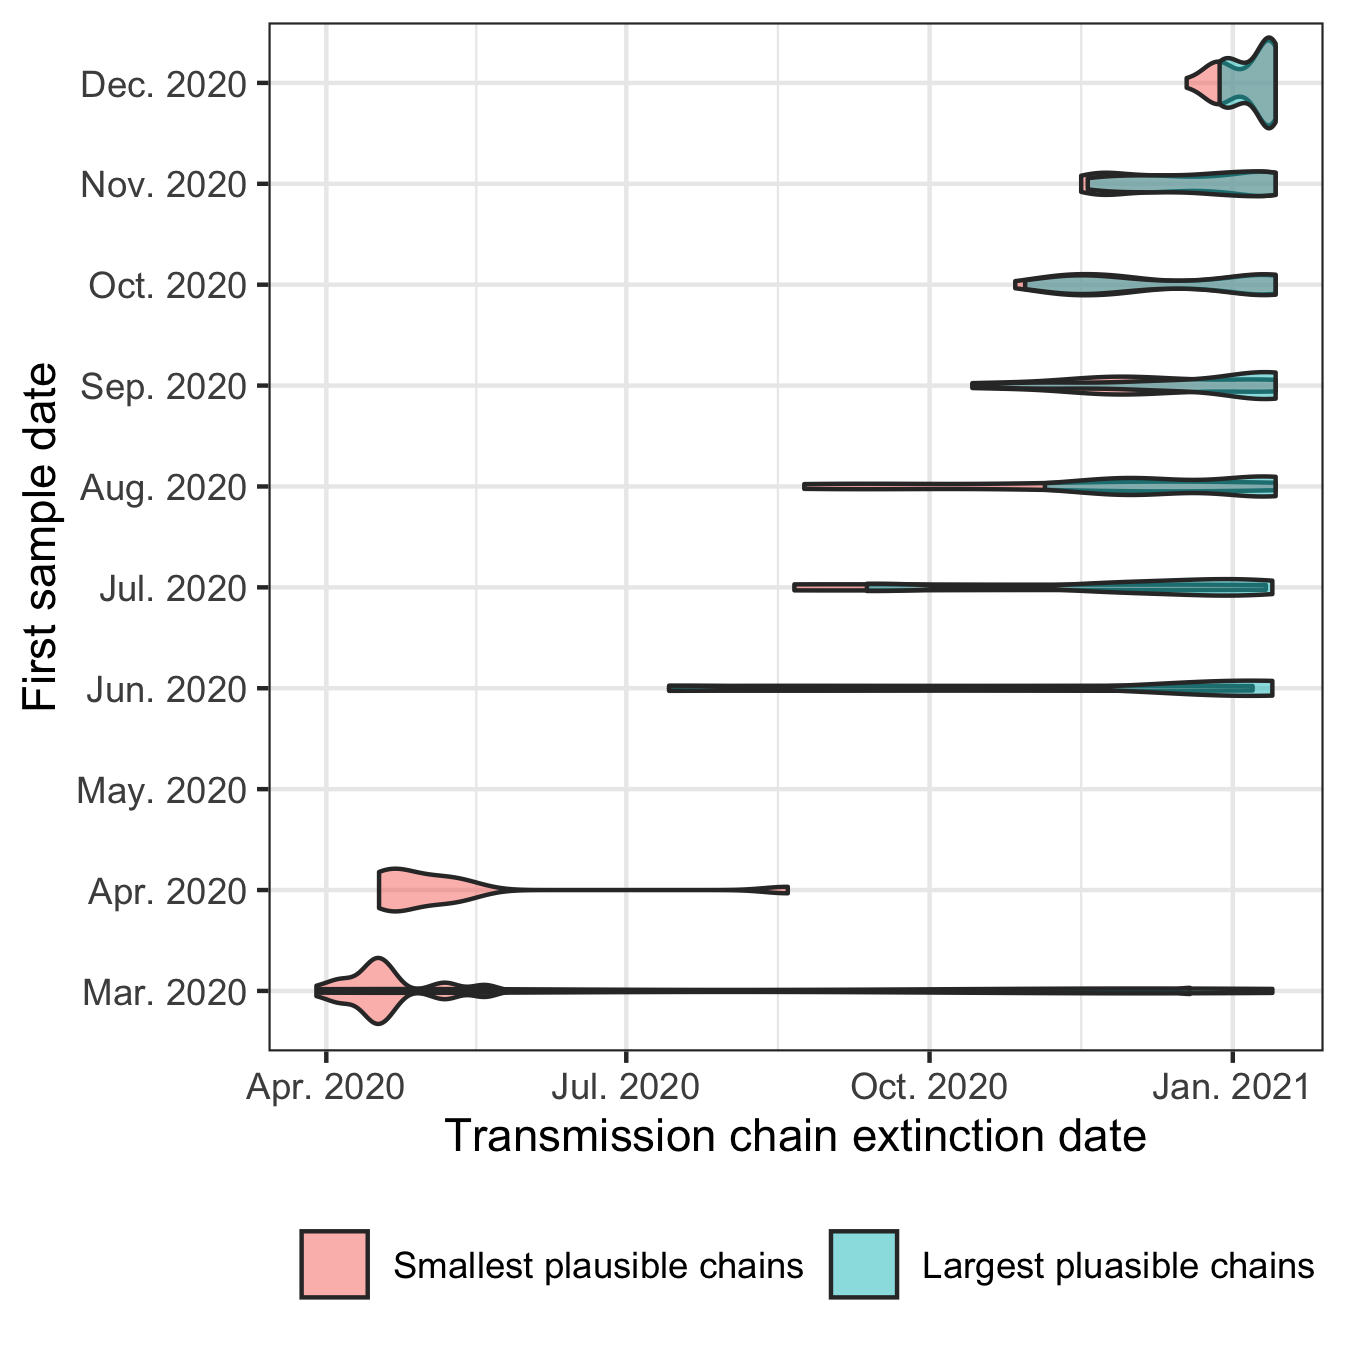
\includegraphics[width=.8\linewidth]{figures/fig_1_chain_longevity.png}
\caption{Detection dates and longevity of Swiss transmission chains.}
\label{fig:chain-description}
\end{figure}

\begin{figure}[tbhp]
\centering
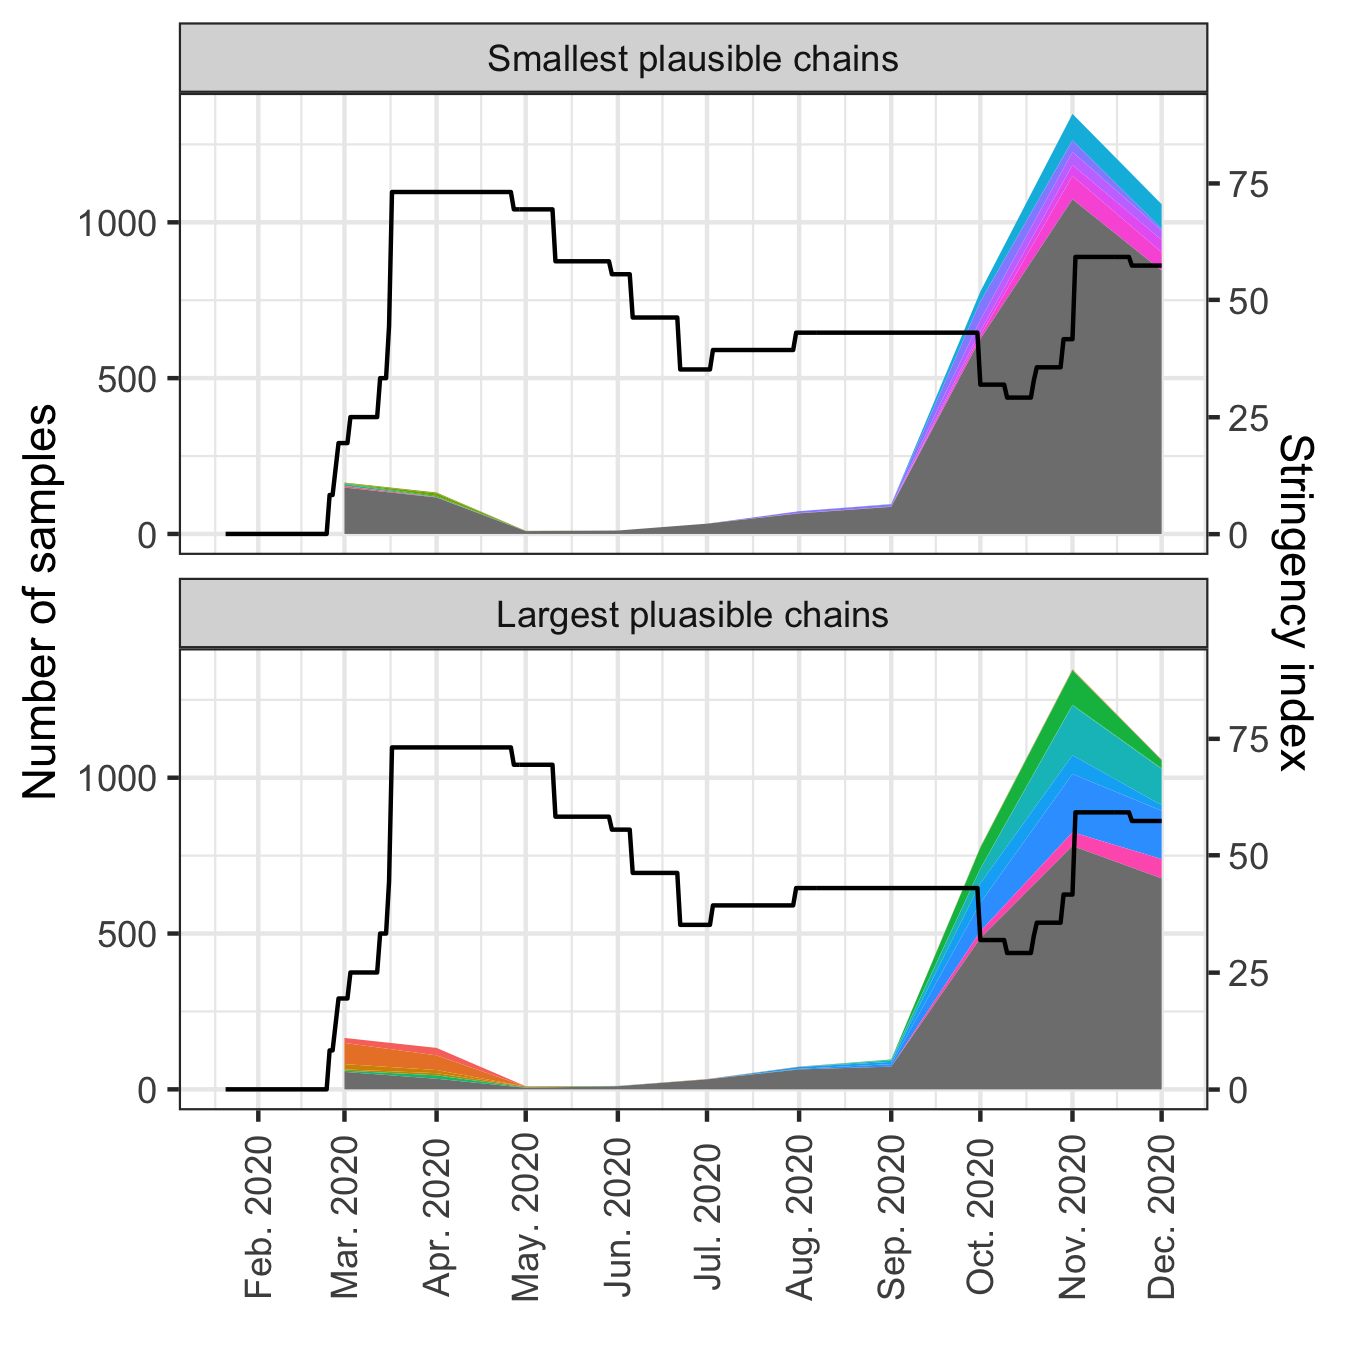
\includegraphics[width=.8\linewidth]{figures/fig_1_chains_through_time.png}
\caption{Size of sampled Swiss transmission chains through time, compared with the Oxford COVID-19 Government Response Tracker stringency index provided by https://ourworldindata.org/grapher/covid-stringency-index. The 5 largest transmission chains during each epidemic wave are highlighted.}  
\label{fig:chain-description-v2}
\end{figure}

\subsection{Transmission chain origins}

\begin{figure}[tbhp]
\centering
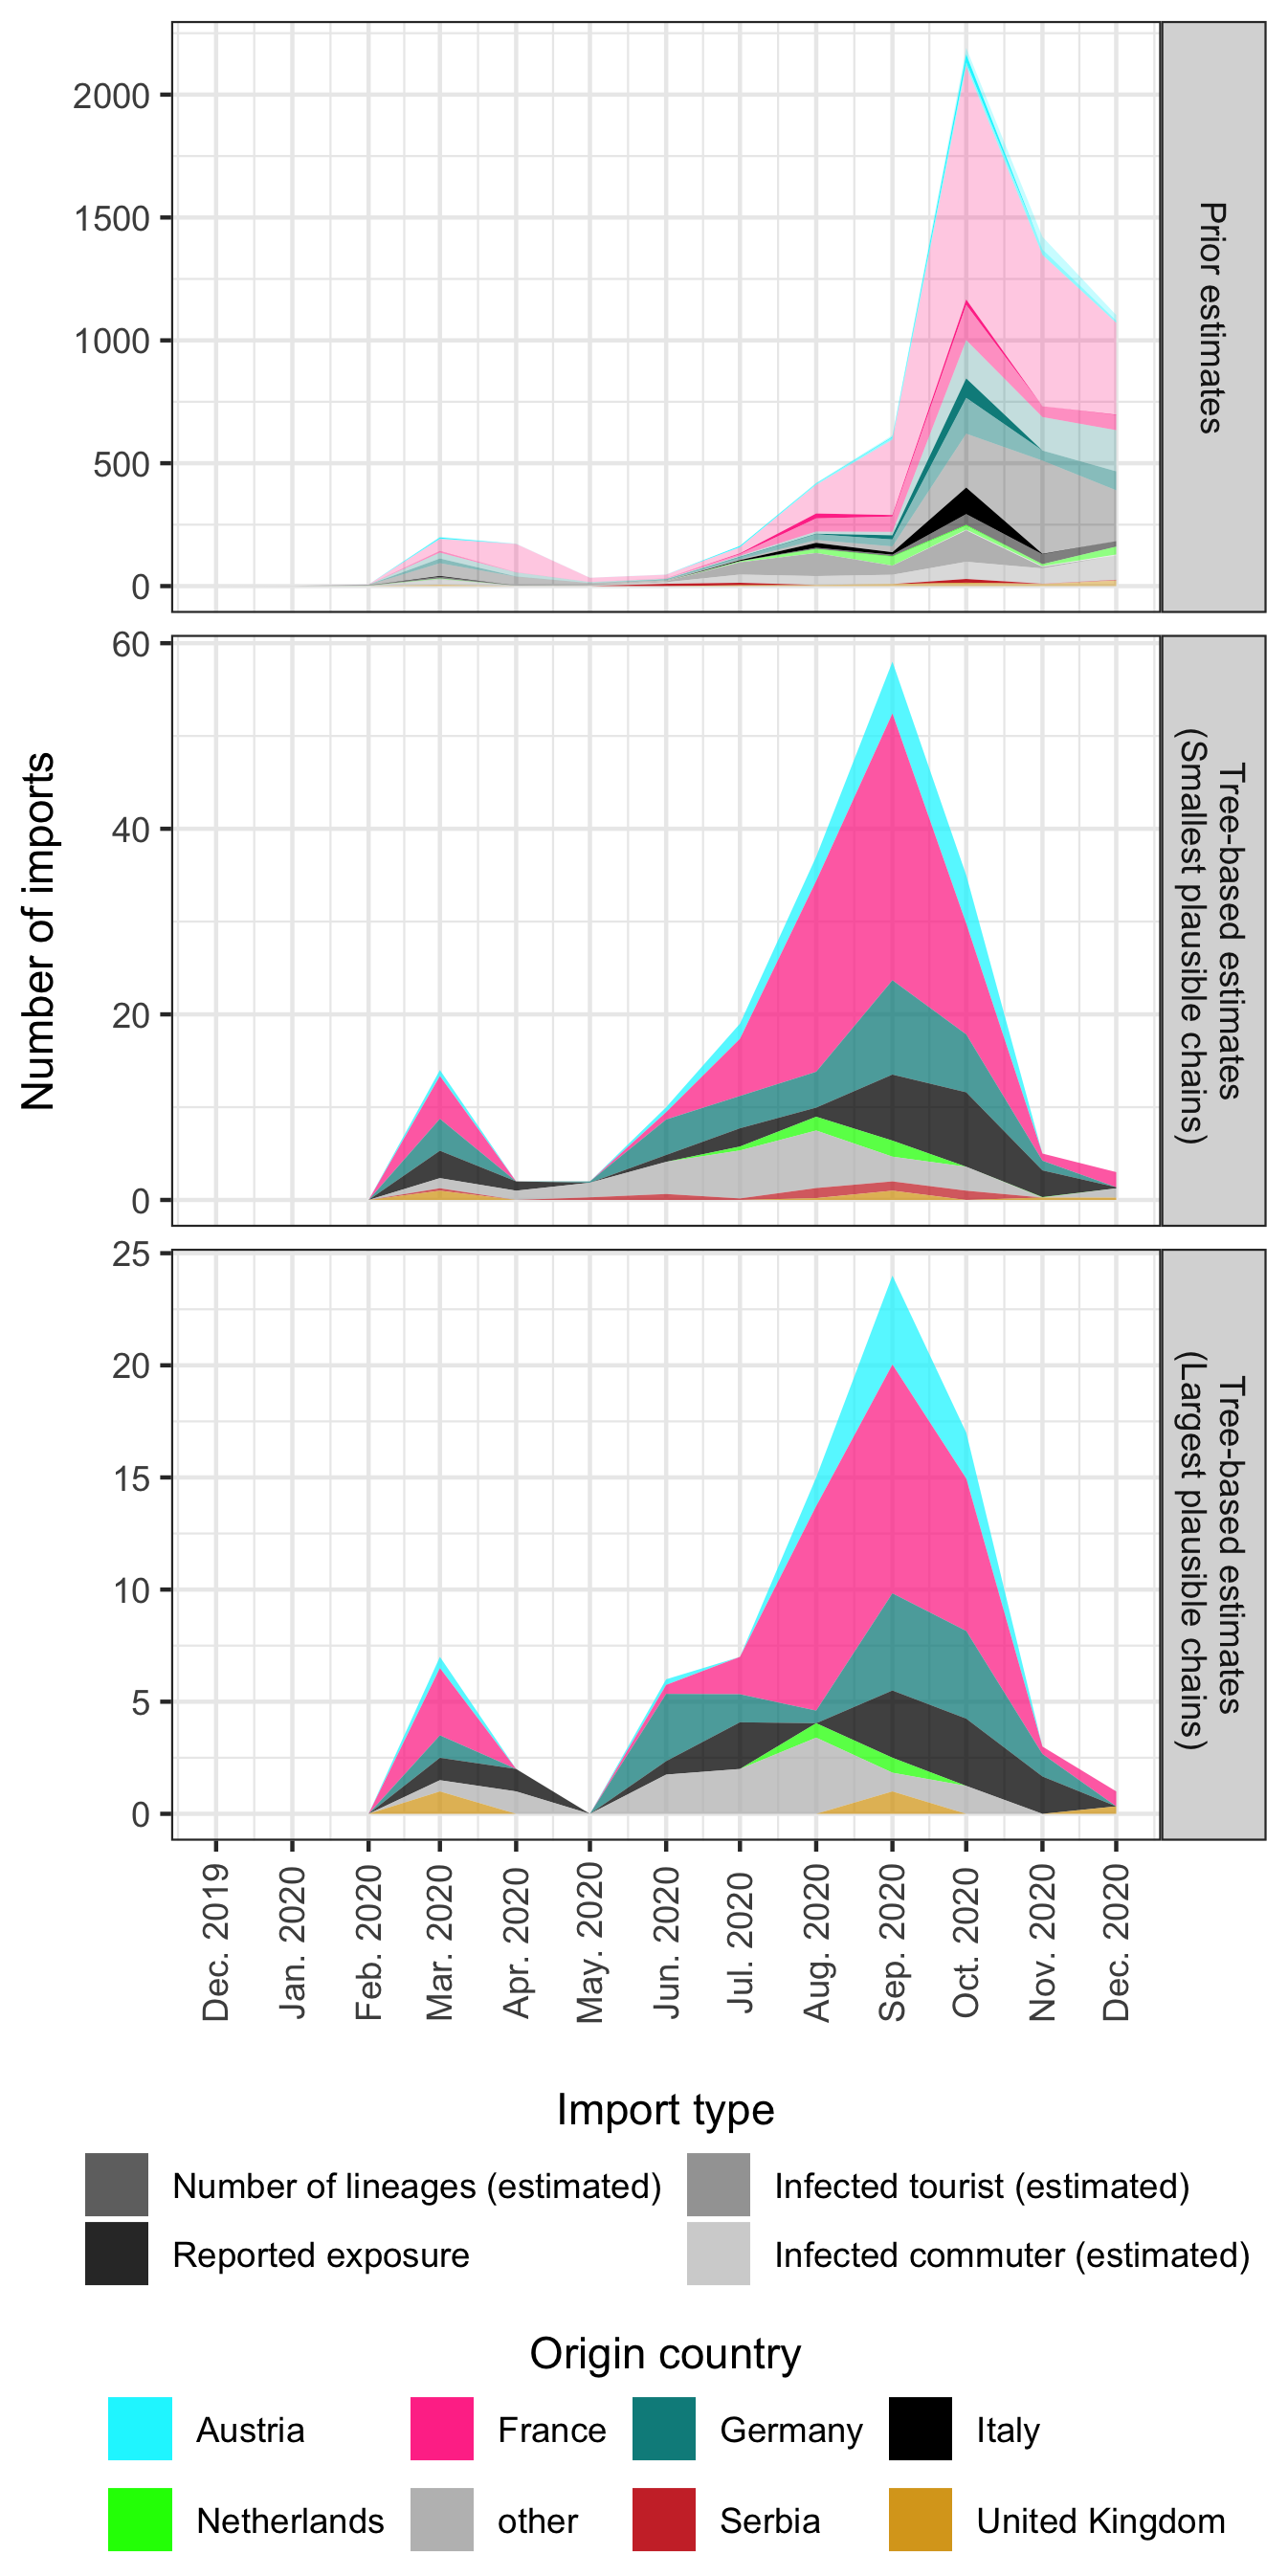
\includegraphics[width=.8\linewidth]{figures/fig_2_chain_origins.png}
\caption{Estimated number of infectious individuals arriving in Switzerland by month and origin country. Prior estimates are based on Swiss FOPH (Federal Office of Public Health) line-list data for foreign exposure locations (Reported exposure), cross-border commuter permit numbers (Infected commuter), and tourist arrivals at Swiss hotels (Infected tourist). Tree-based estimates are parsimony-based estimates of ancestral node locations for nodes ancestral to Swiss transmission chains. For the parsimony-based estimation of ancestral node locations, foreign tips in the tree were chosen proportionally to the prior estimates each month.}  
\label{fig:chain-description-v2}
\end{figure}

\section*{Effect of travel quarantine policy to limit introductions}



\section*{Effect of non-pharmaceutical interventions to limit local transmission}

% \subsection*{Author Affiliations}

% Include department, institution, and complete address, with the ZIP/postal code, for each author. Use lower case letters to match authors with institutions, as shown in the example. PNAS strongly encourages authors to supply an \href{https://orcid.org/}{ORCID identifier} for each author. Individual authors must link their ORCID account to their PNAS account at \href{http://www.pnascentral.org/}{www.pnascentral.org}. For proper authentication, authors must provide their ORCID at submission and are not permitted to add ORCIDs on proofs.

% \subsection*{Submitting Manuscripts}

% All authors must submit their articles at \href{http://www.pnascentral.org/cgi-bin/main.plex}{PNAScentral}. If you are using Overleaf to write your article, you can use the ``Submit to PNAS'' option in the top bar of the editor window. 

% \subsection*{Format}

% Many authors find it useful to organize their manuscripts with the following order of sections;  title, author line and affiliations, keywords, abstract, significance statement, introduction, results, discussion, materials and methods, acknowledgments, and references. Other orders and headings are permitted.

% \subsection*{Manuscript Length}

% A standard 6-page article is approximately 4,000 words, 50 references, and 4 medium-size graphical elements (i.e., figures and tables). The preferred length of articles remains at 6 pages, but PNAS will allow articles up to a maximum of 12 pages.

% \subsection*{References}

% References should be cited in numerical order as they appear in text; this will be done automatically via bibtex, e.g. \cite{belkin2002using} and \cite{berard1994embedding,coifman2005geometric}. All references cited in the main text should be included in the main manuscript file.

% \subsection*{Data Archival}

% PNAS must be able to archive the data essential to a published article. Where such archiving is not possible, deposition of data in public databases, such as GenBank, ArrayExpress, Protein Data Bank, Unidata, and others outlined in the \href{https://www.pnas.org/page/authors/journal-policies#xi}{Information for Authors}, is acceptable.

% \subsection*{Language-Editing Services}
% Prior to submission, authors who believe their manuscripts would benefit from professional editing are encouraged to use a language-editing service (see list at www.pnas.org/page/authors/language-editing). PNAS does not take responsibility for or endorse these services, and their use has no bearing on acceptance of a manuscript for publication. 

% \begin{figure}%[tbhp]
% \centering
% 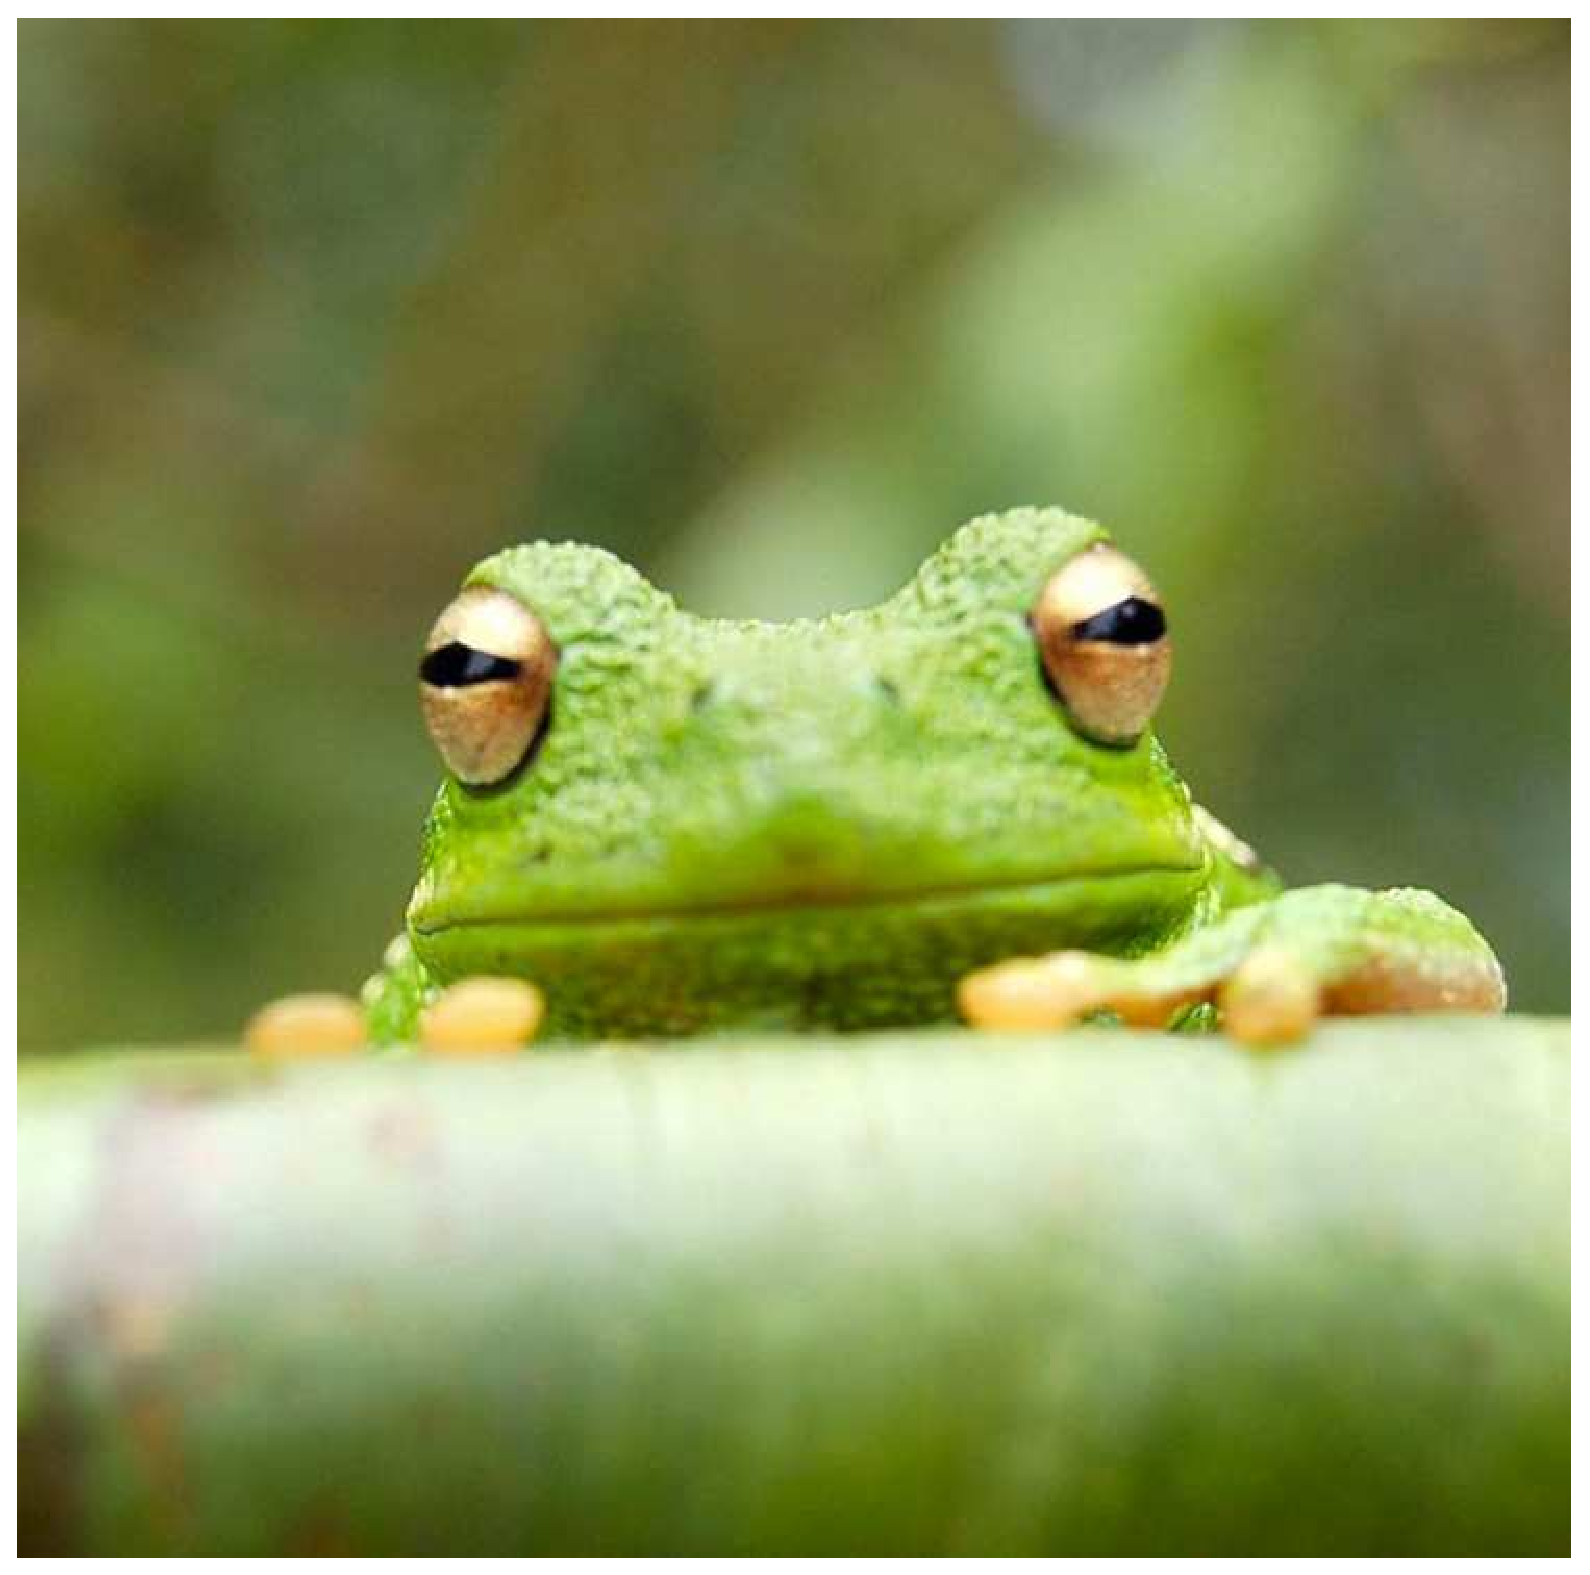
\includegraphics[width=.8\linewidth]{frog}
% \caption{Placeholder image of a frog with a long example legend to show justification setting.}
% \label{fig:frog}
% \end{figure}


% \begin{SCfigure*}[\sidecaptionrelwidth][t]
% \centering
% 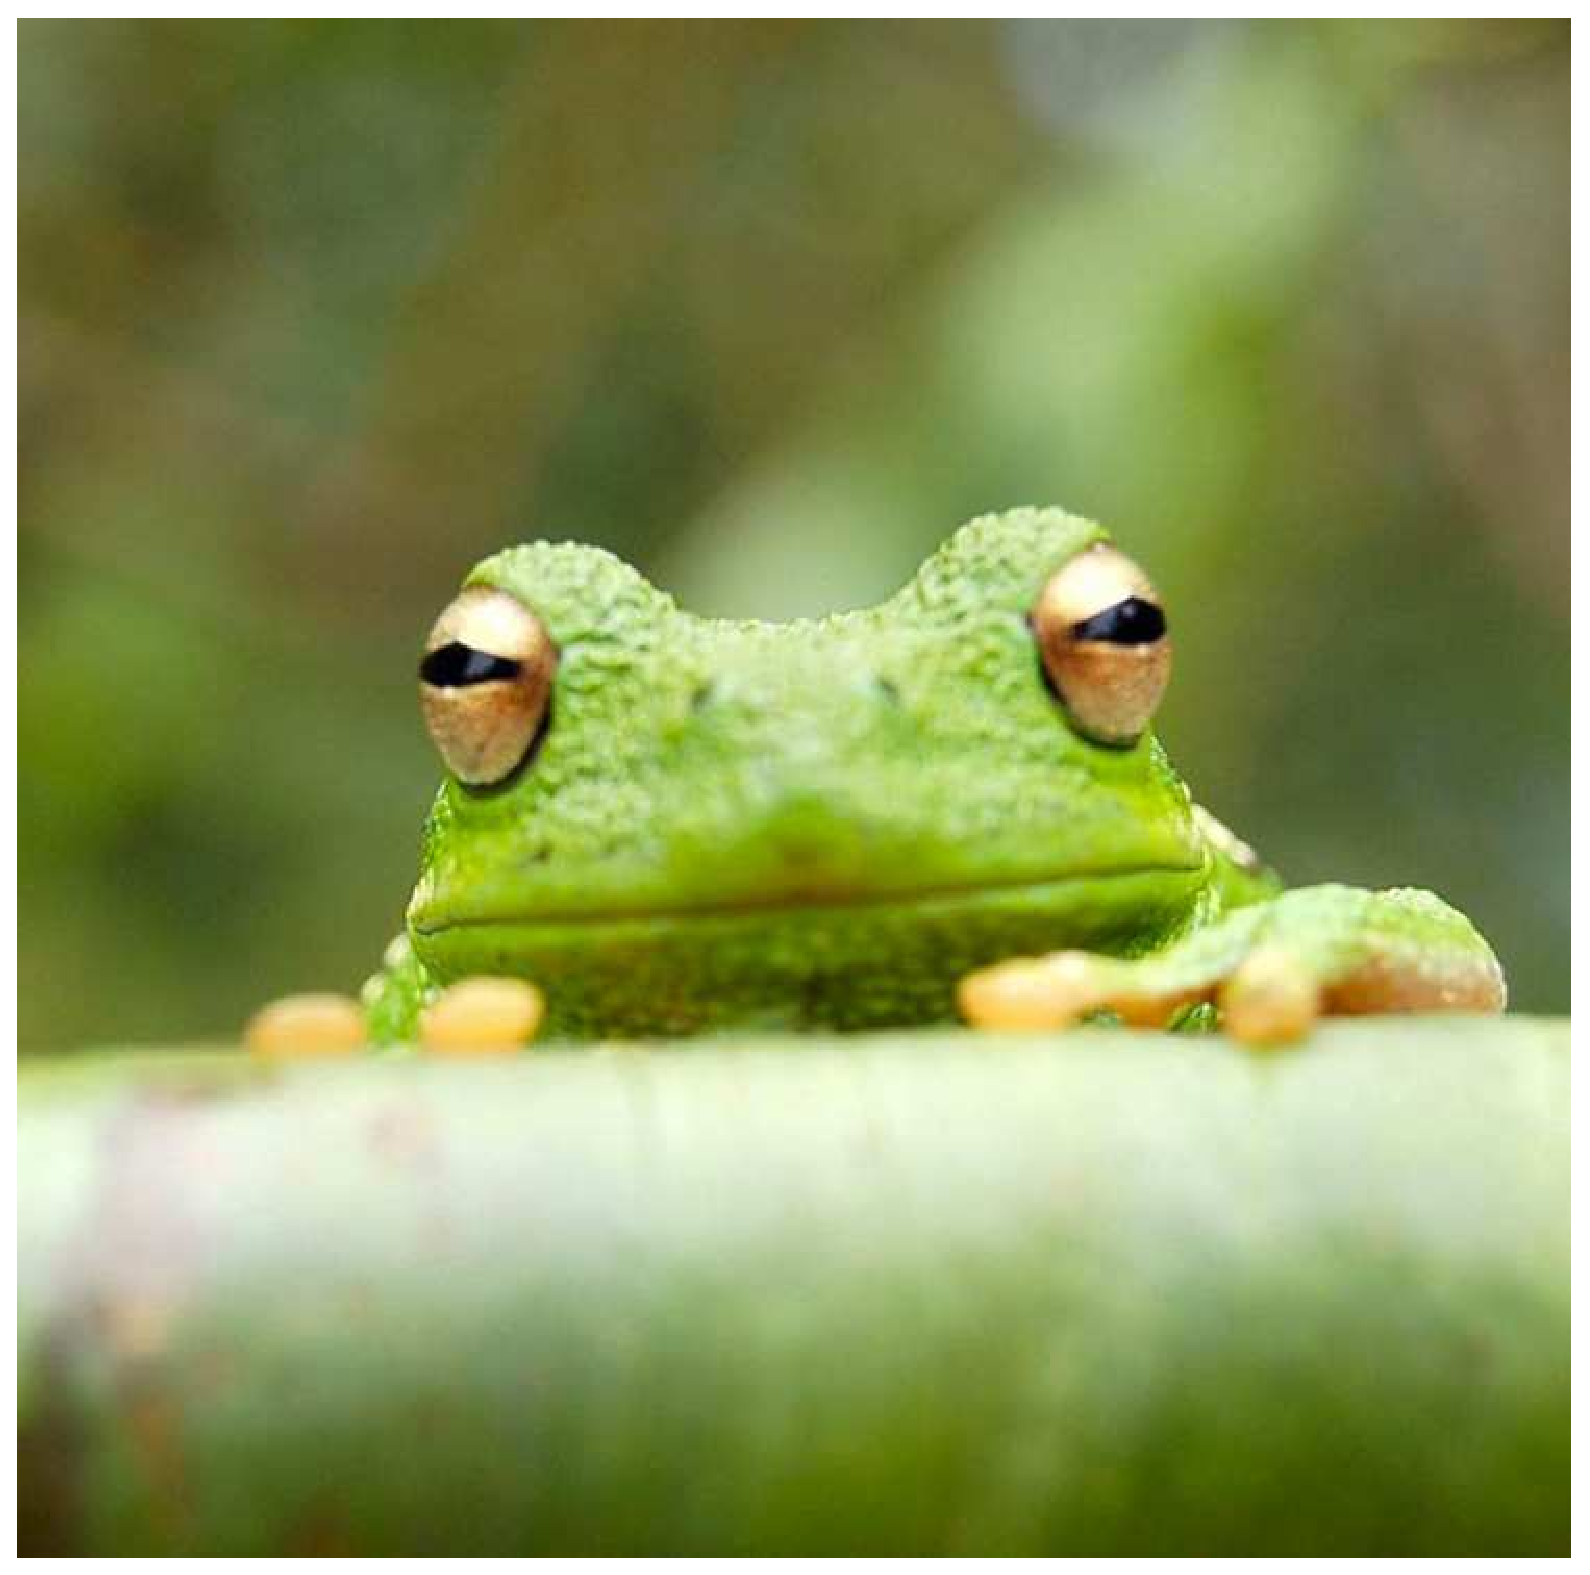
\includegraphics[width=11.4cm,height=11.4cm]{frog}
% \caption{This legend would be placed at the side of the figure, rather than below it.}\label{fig:side}
% \end{SCfigure*}

% \subsection*{Digital Figures}

% EPS, high-resolution PDF, and PowerPoint are preferred formats for figures that will be used in the main manuscript. Authors may submit PRC or U3D files for 3D images; these must be accompanied by 2D representations in TIFF, EPS, or high-resolution PDF format. Color images must be in RGB (red, green, blue) mode. Include the font files for any text.

% Images must be provided at final size, preferably 1 column width (8.7cm). Figures wider than 1 column should be sized to 11.4cm or 17.8cm wide. Numbers, letters, and symbols should be no smaller than 6 points (2mm) and no larger than 12 points (6mm) after reduction and must be consistent. 

% Figures and tables should be labelled and referenced in the standard way using the \verb|\label{}| and \verb|\ref{}| commands.

% Figure \ref{fig:frog} shows an example of how to insert a column-wide figure. To insert a figure wider than one column, please use the \verb|\begin{figure*}...\end{figure*}| environment. Figures wider than one column should be sized to 11.4 cm or 17.8 cm wide. Use \verb|\begin{SCfigure*}...\end{SCfigure*}| for a wide figure with side legends.

% \subsection*{Tables}
% Tables should be included in the main manuscript file and should not be uploaded separately.

% \subsection*{Single column equations}

% Authors may use 1- or 2-column equations in their article, according to their preference.

% To allow an equation to span both columns, use the \verb|\begin{figure*}...\end{figure*}| environment mentioned above for figures.

% Note that the use of the \verb|widetext| environment for equations is not recommended, and should not be used. 

% \begin{figure*}[bt!]
% \begin{align*}
% (x+y)^3&=(x+y)(x+y)^2\\
%       &=(x+y)(x^2+2xy+y^2) \numberthis \label{eqn:example} \\
%       &=x^3+3x^2y+3xy^3+x^3. 
% \end{align*}
% \end{figure*}


% \begin{table}%[tbhp]
% \centering
% \caption{Comparison of the fitted potential energy surfaces and ab initio benchmark electronic energy calculations}
% \begin{tabular}{lrrr}
% Species & CBS & CV & G3 \\
% \midrule
% 1. Acetaldehyde & 0.0 & 0.0 & 0.0 \\
% 2. Vinyl alcohol & 9.1 & 9.6 & 13.5 \\
% 3. Hydroxyethylidene & 50.8 & 51.2 & 54.0\\
% \bottomrule
% \end{tabular}

% \addtabletext{nomenclature for the TSs refers to the numbered species in the table.}
% \end{table}

% \subsection*{Supporting Information Appendix (SI)}

% Authors should submit SI as a single separate SI Appendix PDF file, combining all text, figures, tables, movie legends, and SI references. SI will be published as provided by the authors; it will not be edited or composed. Additional details can be found in the \href{https://www.pnas.org/authors/submitting-your-manuscript#manuscript-formatting-guidelines}{PNAS Author Center}. The PNAS Overleaf SI template can be found \href{https://www.overleaf.com/latex/templates/pnas-template-for-supplementary-information/wqfsfqwyjtsd}{here}. Refer to the SI Appendix in the manuscript at an appropriate point in the text. Number supporting figures and tables starting with S1, S2, etc.

% Authors who place detailed materials and methods in an SI Appendix must provide sufficient detail in the main text methods to enable a reader to follow the logic of the procedures and results and also must reference the SI methods. If a paper is fundamentally a study of a new method or technique, then the methods must be described completely in the main text.

% \subsubsection*{SI Datasets} 

% Supply .xlsx, .csv, .txt, .rtf, or .pdf files. This file type will be published in raw format and will not be edited or composed.


% \subsubsection*{SI Movies}

% Supply Audio Video Interleave (avi), Quicktime (mov), Windows Media (wmv), animated GIF (gif), or MPEG files. Movie legends should be included in the SI Appendix file. All movies should be submitted at the desired reproduction size and length. Movies should be no more than 10MB in size.


% \subsubsection*{3D Figures}

% Supply a composable U3D or PRC file so that it may be edited and composed. Authors may submit a PDF file but please note it will be published in raw format and will not be edited or composed.


\matmethods{Please describe your materials and methods here. This can be more than one paragraph, and may contain subsections and equations as required. 

\subsection*{Subsection for Method}
Example text for subsection.
}

\showmatmethods{} % Display the Materials and Methods section

\acknow{Please include your acknowledgments here, set in a single paragraph. Please do not include any acknowledgments in the Supporting Information, or anywhere else in the manuscript.}

\showacknow{} % Display the acknowledgments section

% Bibliography
\bibliography{pnas-sample}

\end{document}
